
\subsection*{Projedeki yeri ve araç seçimi}
Sionna, NVIDIA'nın açık kaynaklı bağlantı düzeyi (link-level) simülatör kütüphanesidir; \textbf{Sionna RT} ise ışın izleme (ray tracing) ile gerçek bir şehir sahnesinde kanalı hesaplar. Projede Sionna \textbf{kazanç tarafını} ölçer: sensing'e ayrılan kaynak payı $\alpha$ arttıkça bir İHA'yı hangi mesafeden, ne olasılıkla ve ne doğrulukla bulabiliyoruz? Sionna RT, binaların görüş hattını kestiği gerçekçi bir senaryo (Münih sahnesi, 4,9\,GHz) sağlıyor. ns-3 ve OCUDU yalnızca bedeli ölçtüğü için, kazanç ölçülmeden ödünleşim (trade-off) çıkmaz.

\subsection*{Kurulum}
Kurulum iki ortamda yapıldı ve ikisinde de aynı paket sürümleri elde edildi.
\begin{center}\sffamily\small
\begin{tabular}{@{}lll@{}}
\toprule
 & \textbf{Ortam A: Ubuntu} & \textbf{Ortam B: Windows} \\
\midrule
İşletim sistemi & Ubuntu 22.04.5 LTS & Windows 11 \\
Python & sistem Python'u 3.10.12 & 3.11.9 (sanal ortam) \\
LLVM (Sionna RT için) & \texttt{libllvm14} (apt) & LLVM 23.1.3 (\texttt{winget}) \\
Sionna / sionna-rt & 1.2.2 / 1.2.2 & 1.2.2 / 1.2.2 \\
TensorFlow, Mitsuba, Dr.Jit & 2.21.0, 3.8.0, 1.3.1 & 2.21.0, 3.8.0, 1.3.1 \\
Süre ve disk & $\approx$5 dk (hızlı ağda), 2,8 GB & 15--30 dk, 2,1 GB \\
\bottomrule
\end{tabular}
\end{center}
\textbf{Ortam A (Ubuntu) komutları} (ayrıntı: \texttt{kurulum/03-sionna-ubuntu.md}):
\begin{lstlisting}
sudo apt update
sudo apt install -y python3-venv libllvm14 libatomic1
mkdir -p ~/venvs && python3 -m venv ~/venvs/ehb415
~/venvs/ehb415/bin/python -m pip install --upgrade pip
~/venvs/ehb415/bin/python -m pip install --retries 10 --timeout 60 "sionna==1.2.2" jupyterlab matplotlib scipy
\end{lstlisting}
\textbf{Ortam B (Windows) komutları} (PowerShell; ayrıntı: \texttt{kurulum/03-sionna-windows.md}). LLVM kurulumu \emph{yönetici} PowerShell ister:
\begin{lstlisting}
python -m venv C:\Users\$env:USERNAME\venvs\ehb415
C:\Users\$env:USERNAME\venvs\ehb415\Scripts\python.exe -m pip install --retries 10 --timeout 60 "sionna==1.2.2" jupyterlab matplotlib scipy
.\kur-llvm.ps1      # yonetici PowerShell: LLVM kurar ve DRJIT_LIBLLVM_PATH ayarlar
\end{lstlisting}
\texttt{sionna==1.2.2} sürümünü sabitlemek önemli: Python 3.11'de sürümsüz \texttt{pip install sionna} Sionna 2.2.0'ı seçer ve bizim betiklerimiz 1.2.2 içindir.

\subsection*{Karşılaşılan sorunlar ve çözümleri}
\begingroup\sffamily\small
\begin{xltabular}{\textwidth}{@{}p{4.4cm}X@{}}
\toprule
\textbf{Sorun} & \textbf{Neden ve çözüm} \\
\midrule
\texttt{ensurepip is not available} (Ubuntu) & \texttt{python3-venv} paketi yok. \texttt{sudo apt install -y python3-venv}. \\
\texttt{Could not import the Dr.Jit binary extension ... incompatible with the current interpreter} (Ubuntu) & Mesaj yanıltıcı: asıl neden Python sürümü değil, \texttt{libatomic.so.1} eksikliği. \texttt{sudo apt install -y libatomic1}. \\
\texttt{LLVM shared library ("libLLVM.so") could not be found} (Ubuntu) & \texttt{sudo apt install -y libllvm14}. \\
\texttt{LLVM-C.dll could not be found} (Windows) & LLVM kurulu değil ya da \texttt{DRJIT\_LIBLLVM\_PATH} ayarsız. \texttt{kur-llvm.ps1} (yönetici) çalıştırılır ve \textbf{yeni bir PowerShell} açılır (ortam değişkeni eski pencerelere yansımaz). \\
Sonda \texttt{free(): invalid pointer} veya \texttt{Segmentation fault} (Ubuntu) & TensorFlow, \texttt{sionna.rt}'den önce içe aktarılmış. \texttt{import sionna.rt} her zaman \textbf{ilk} satır olmalı. Windows'ta bu sorun yok. \\
Python 3.11'de beklenmedik Sionna 2.2.0 kurulumu & Sürüm sabitlenmemişti. \texttt{"sionna==1.2.2"} yazılır. \\
\texttt{TypeError: PathSolver ... 'samples\_per\_tx'} & Sionna 1.2.2'de parametre adı \texttt{samples\_per\_src}'dir; eski örnek kodlarda farklı geçer. \\
\texttt{TensorFlow GPU support is not available on native Windows} & Beklenen ve zararsız uyarı; Sionna CPU'da çalışır. \\
\bottomrule
\end{xltabular}
\endgroup

\subsection*{Örnek çalıştırma}
\subsubsection*{Kurulum doğrulaması (Ortam B, Windows)}
Önce paket sürümlerini listeledim, ardından iki doğrulama betiğini çalıştırdım: \texttt{sionna\_dogrulama.py} saf NumPy ile tek hedefli bir OFDM radar testi yapar ve Sionna'nın \texttt{ResourceGrid} nesnesini oluşturur; \texttt{sionna\_rt\_dogrulama.py} ise Münih sahnesini yükleyip ışın yollarını hesaplar.
\begin{figure}[h!]
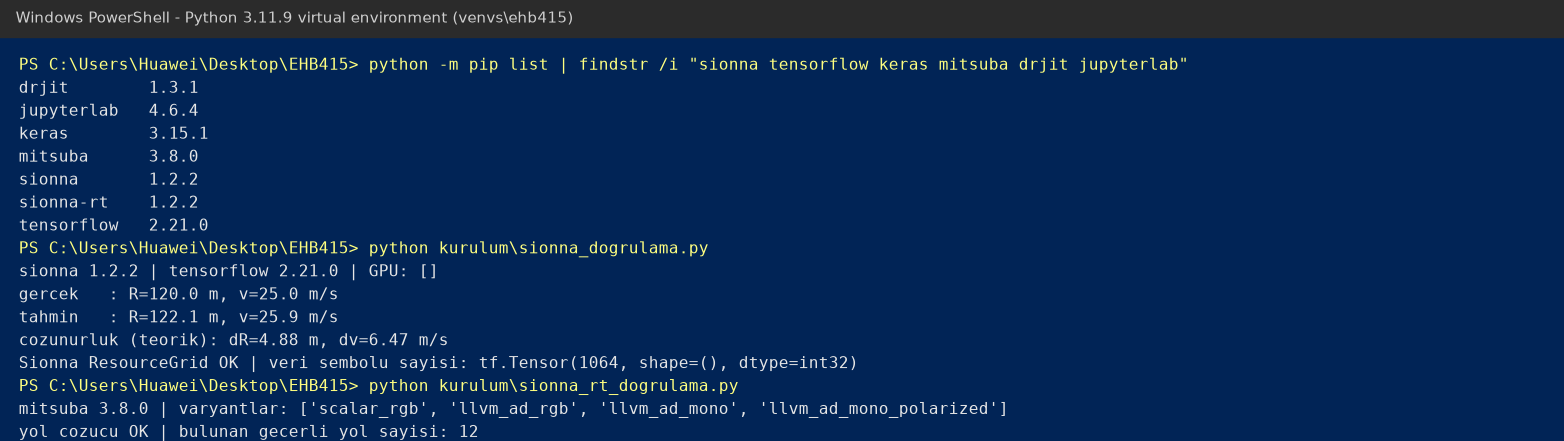
\includegraphics[width=\textwidth]{img/sionna_windows_terminal.png}
\caption{Paket sürümleri ve iki doğrulama betiğinin çıktısı (Windows PowerShell).}
\end{figure}
Radar testinde gerçek hedef 120,0\,m ve 25,0\,m/s iken tahmin 122,1\,m ve 25,9\,m/s çıktı; hatalar teorik çözünürlük hücresinin (4,88\,m ve 6,47\,m/s) içinde olduğundan sonuç doğrudur. Sionna RT 12 geçerli ışın yolu buldu.

\subsubsection*{Proje betikleri (Ortam A, Ubuntu)}
Ubuntu ortamında projenin iki betiğini çalıştırdım: \texttt{radar\_takip.py}, sembollerin $\alpha$ kadarını sensing'e ayıran basit bir radar modeliyle farklı mesafelerdeki bir İHA'yı tespit ediyor; \texttt{rt\_sehir.py} ise Sionna RT ile şehir sahnesinde radyo haritasını ve ışın yollarını hesaplıyor.
\begin{figure}[h!]
\centering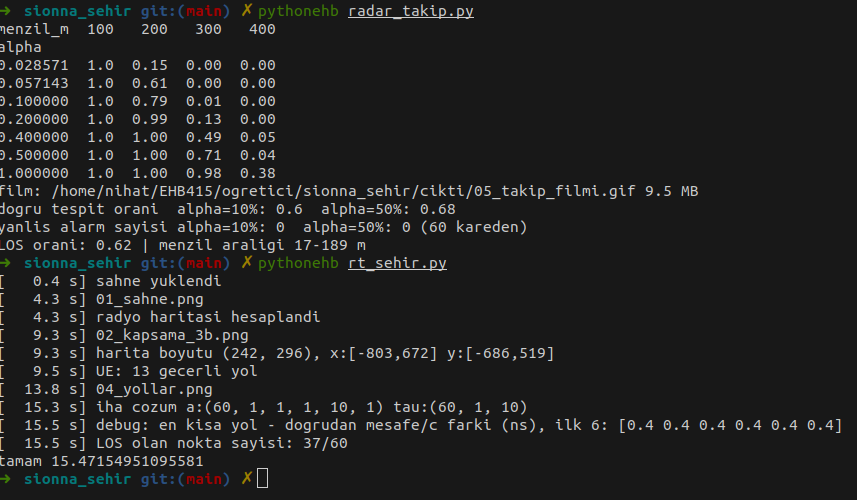
\includegraphics[width=0.78\textwidth]{img/sionna_ubuntu_terminal.png}
\caption{\texttt{radar\_takip.py} tespit olasılığı tablosu ve \texttt{rt\_sehir.py} çıktısı (Ubuntu).}
\end{figure}
\begin{itemize}
\item \textbf{Tespit olasılığı:} 100\,m'de $\alpha$ ne olursa olsun İHA bulunuyor. 200\,m'de $\alpha=\%2{,}9$ için 0,15, $\alpha=\%20$ için 0,99. 300\,m'de ancak $\alpha=\%100$'de 0,98; 400\,m'de en fazla 0,38.
\item \textbf{Takip senaryosu (60 kare):} doğru tespit oranı $\alpha=\%10$ için 0,60, $\alpha=\%50$ için 0,68; yanlış alarm yok.
\item \textbf{Görüş hattı:} 60 noktanın 37'sinde (\%62) İHA ile verici arasında doğrudan görüş var. Tespit oranlarının bu orana yakın çıkması, tespitin büyük ölçüde doğrudan görüş olan karelerden geldiğini düşündürüyor.
\item \textbf{Sionna RT süresi:} sahne 0,4\,s'de yüklendi, tüm adımlar yaklaşık 15,5\,s'de bitti.
\end{itemize}
\begin{figure}[h!]
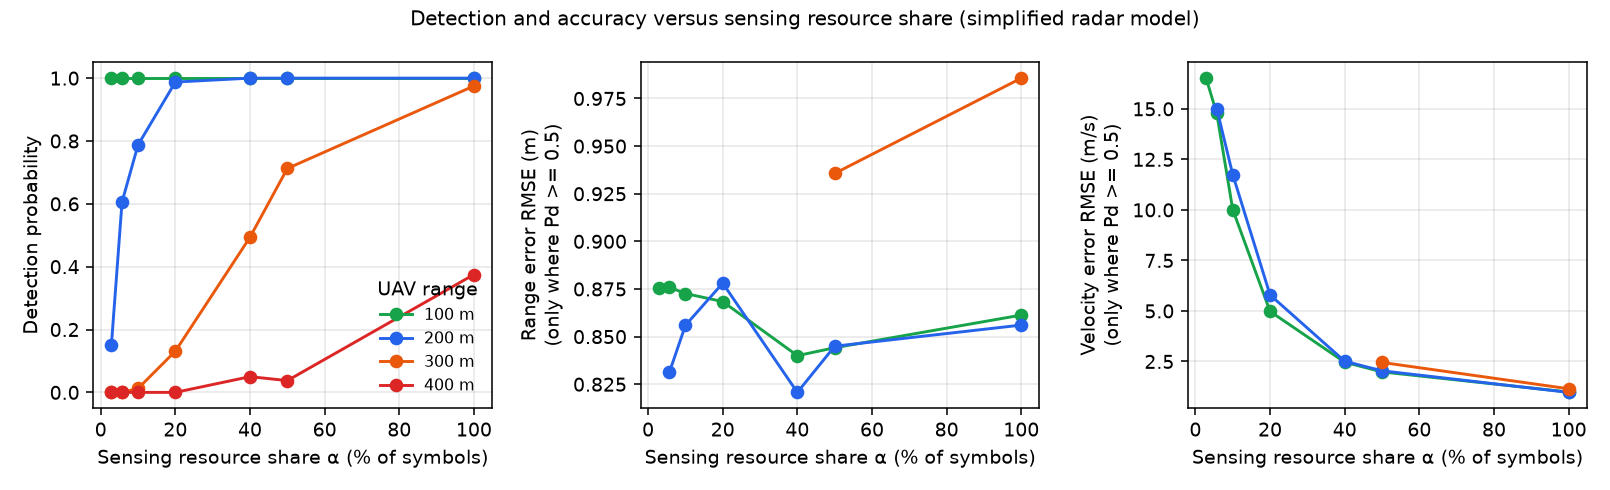
\includegraphics[width=\textwidth]{img/sionna_grafik.png}
\caption{Sensing payı $\alpha$ arttıkça tespit olasılığı, menzil hatası ve hız hatası.}
\end{figure}
Grafikte menzil hatası $\alpha$'dan neredeyse bağımsız ($\approx$0,8--1,0\,m); hız hatası ise $\alpha$ arttıkça 15--16\,m/s'den yaklaşık 1\,m/s'ye düşüyor. Menzil çözünürlüğü sembol sayısına değil bant genişliğine bağlı olduğu için menzil doğruluğu pek değişmiyor; sensing'e daha çok sembol ayırmak özellikle hız (Doppler) kestirimini iyileştiriyor.
\begin{figure}[h!]
\centering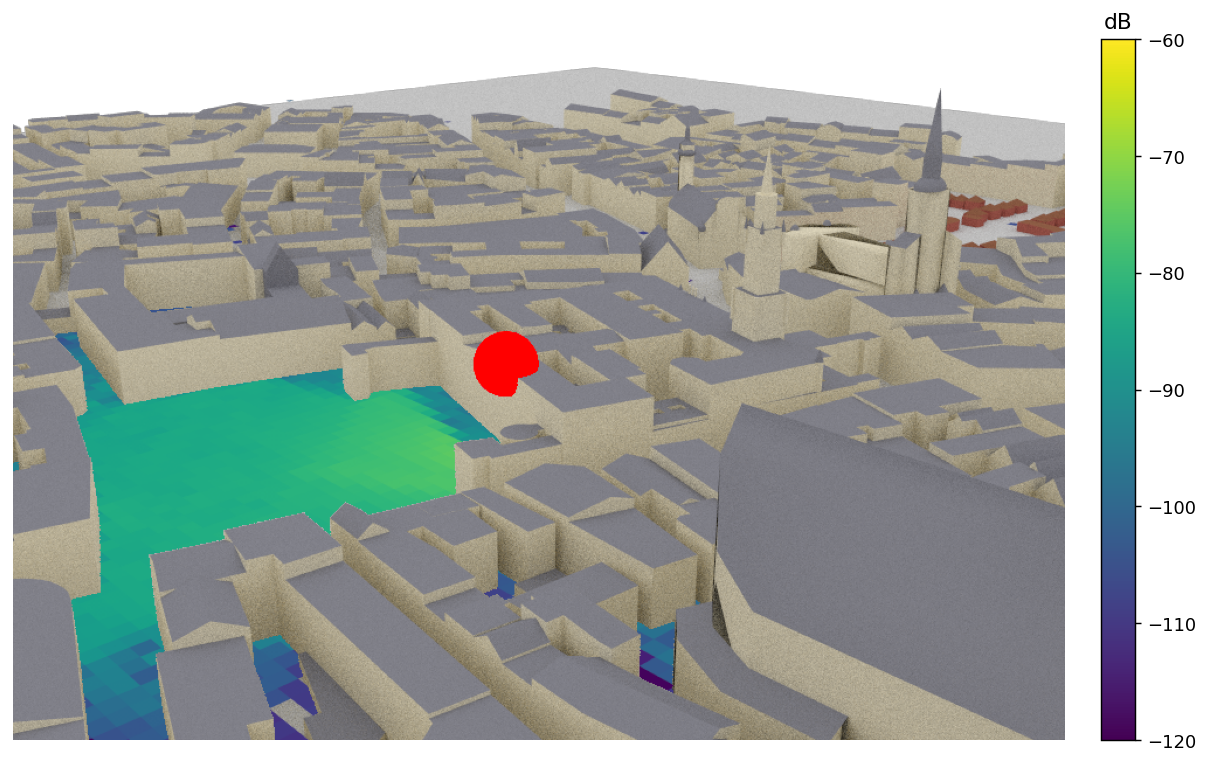
\includegraphics[width=0.62\textwidth]{img/sionna_kapsama3b.png}
\caption{Sionna RT ile hesaplanan radyo haritası (yol kazancı, dB). Kırmızı küre vericinin (gNB) konumu; binaların arkasında sinyal belirgin biçimde zayıflıyor.}
\end{figure}

\subsection*{Değerlendirme ve sonraki adımlar}
Sionna 1.2.2 ve Sionna RT iki farklı ortamda (Ubuntu 22.04 ve Windows 11) kuruldu, doğrulama betikleri hatasız bitti ve proje betikleri beklenen sonuçları üretti. Sınırlamalar: GPU kullanılmadı (CPU); radar modeli basitleştirilmiş bir modeldir (``oyuncak radar''), tam bir 3GPP kanal modeli değildir. Sionna RT çıktısını ns-3'e besleyen SioLENA modülü \textbf{denenmedi}. Sonraki adımlar:
\begin{itemize}
\item Radar kodundaki \texttt{radar()} fonksiyonunu (2B FFT ile menzil ve hız kestirimi) satır satır incelemek.
\item Artık öz-girişim (\texttt{X\_SI\_DB}) değerini değiştirip tespit olasılığına etkisini ölçmek.
\item Elde edilen $P_d$ ve hata eğrilerini TR~38.765'in hedefleriyle ($P_{md}\le\%5$) karşılaştırmak.
\end{itemize}
